\section{Erreurs générées}%
\label{sec.results.errors}

Parmi les erreurs générées par chatGPT, 
celles qui ressemblent le plus à des erreurs humaines ont été manuellement sélectionnées.
Le résultat de cette sélection est une liste de 217 mots 
avec une moyenne de 5 erreurs retenues par mot (1104 erreurs en termes absolus).
Ces erreurs ont été analysées et classées en 4 catégories :
\begin{itemize}
    \item des suppressions : de lettres ou de syllabes,
    \item des ajouts : de lettres ou de syllabes,
    \item des substitutions : de lettres ou de syllabes,
    \item des transpositions : de lettres ou de syllabes.
\end{itemize}

\begin{figure}[hbt]
    \centering
    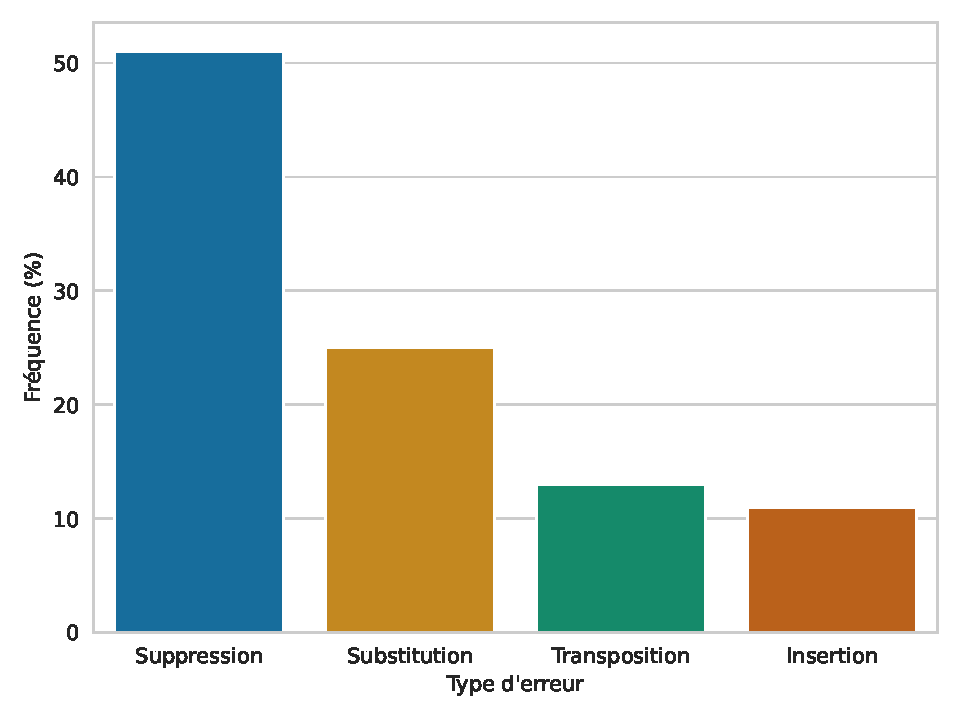
\includegraphics[width=8cm]{assets/python/rules-stats.pdf}
    \caption{Fréquences des catégories d'erreurs}
    \label{fig.errors-freq}
\end{figure}

Les fréquences de ces erreurs (pour les 32 premiers mots qui ont 327 modifications) 
sont présentées dans la Figure~\ref{fig.errors-freq}.
Sur la base de ces fréquences, nous avons créé une fonction qui génère, pour un mot donné,
des erreurs qui suivent les mêmes fréquences (voir le code~\ref{code.errors-generation}).

\begin{lstlisting}[
    language=Python,
    caption={Génération des erreurs pour un mot},
    label={code.errors-generation},
]
def corrupt_word(
    word,
    p_remove=0.51,
    p_substitute=0.25,
    p_transpose=0.13,
    p_insert=0.11,
    p_skip=0.5,
    all_syllables=None,
):
    from random import seed, randint, random
    from hyphen import Hyphenator

    hyphenator = Hyphenator("fr_FR")
    syls = hyphenator.syllables(word)

    # skip words that are too short
    if len(syls) < 3:
        return word

    # skip all words with probability p_skip
    if random() < p_skip:
        return word

    # remove a syllable with probability p_remove
    if random() < p_remove:
        idx = randint(0, len(syls) - 1)
        del syls[idx]

    # substitute a syllable with probability p_substitute
    if random() < p_substitute:
        idx1 = randint(0, len(syls) - 1)
        syls[idx] = choice(all_syllables)

    # transpose two syllables with probability p_transpose
    if random() < p_transpose:
        idx1 = randint(0, len(syls) - 1)
        idx2 = randint(0, len(syls) - 1)
        syls[idx1], syls[idx2] = syls[idx2], syls[idx1]

    # insert a syllable with probability p_insert
    if random() < p_insert:
        idx = randint(0, len(syls) - 1)
        syls.insert(idx, choice(all_syllables))
    return "".join(syls)
\end{lstlisting}

Les erreurs générées par cette fonction sont similaires aux erreurs générées par chatGPT
(par exemple, maintenant \(\to\) temain | tenant, entendu \(\to\) enten | tendu | tenendu.).
Cependant, certaines parmi elles ne sont pas prononçables
(par exemple, maintenant \(\to\) nantmain, simplement \(\to\) mentple).
Pour cette raison, nous avons décidé de ne pas les utiliser dans le corpus.
Cela étant dit, il nous paraît intéressant d'explorer des méthodes de filtrage de ces erreurs.
Si réussies, elles permettent de générer des erreurs plus rapidement et plus facilement que par chatGPT\@.
